\section{Evaluation}



\subsection{Node Inference Attack}


\begin{figure}
    \centering
    \begin{minipage}[b]{1\linewidth}
    \centering
    \subfigure[Prediction Confidence for a particular data record]{
    \label{fig:nonmem_soft_label}
    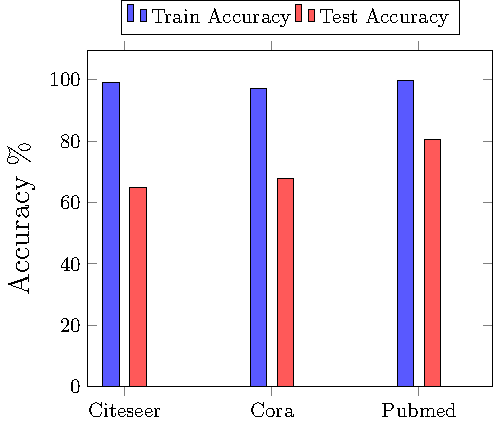
\includegraphics[width=0.5\linewidth,height=3.5cm, keepaspectratio]{figures/BBMIA/GenErr.pdf}
    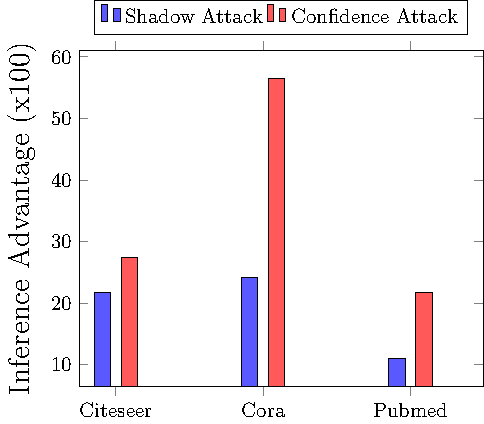
\includegraphics[width=0.5\linewidth,height=3.5cm, keepaspectratio]{figures/BBMIA/NodeIA.pdf}
    }

    \end{minipage}
    \caption{Distribution of the confidence score vectors of the target classifier on the training data and test data of class 29 in the Purchase100 dataset. Each color represents one data record.}
    \label{fig:soft_label}
\end{figure}

Confidence Score
cora
model accuracy for training and test- (0.9722222222222222, 0.6789667896678967)
maximum inference accuracy is: 0.78280032800328
Shadow: 0.6206


citeseer
model accuracy for training and test- (0.9924242424242424, 0.649546827794562)
maximum inference accuracy is: 0.6374
Shadow: 0.6087842167902591

PubMed
model accuracy for training and test- (0.9961928934010152, 0.8059852903880295)
maximum inference accuracy is: 0.6089809609267083
Shadow: 0.5551

\begin{figure}
    \centering
    \begin{minipage}[b]{1\linewidth}
    \centering
    \subfigure[Prediction Confidence for a particular data record]{
    \label{fig:nonmem_soft_label}
    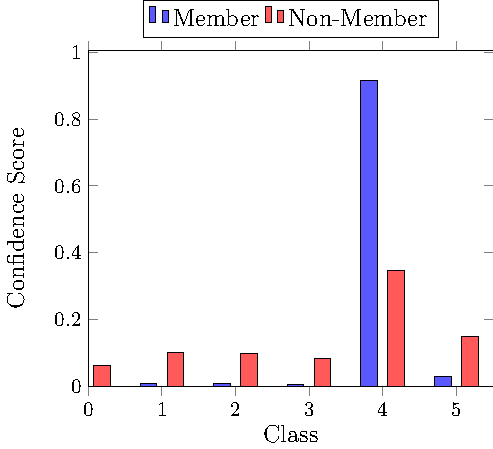
\includegraphics[width=0.5\linewidth]{figures/BBMIA/citeseer_hist.pdf}
    \raisebox{2mm}{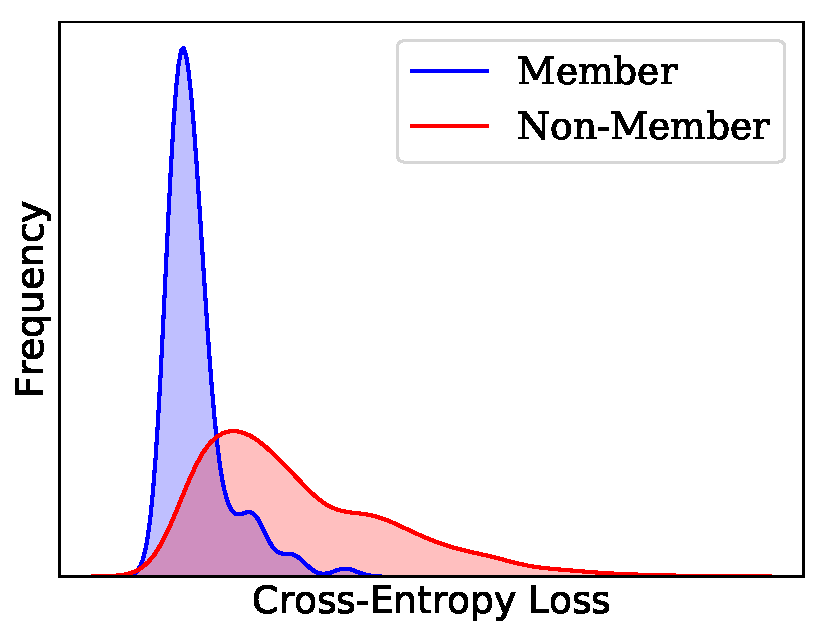
\includegraphics[width=0.5\linewidth]{figures/BBMIA/citeseer.pdf}}
    }

    \subfigure[Output Distribution for all records]{
   	\label{fig:mem_soft_label}
    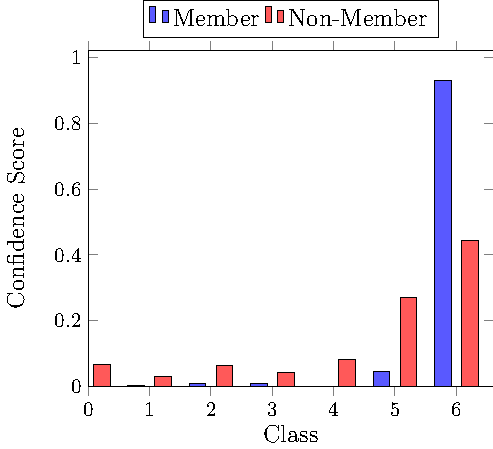
\includegraphics[width=0.5\linewidth]{figures/BBMIA/cora_hist.pdf}
    \raisebox{2mm}{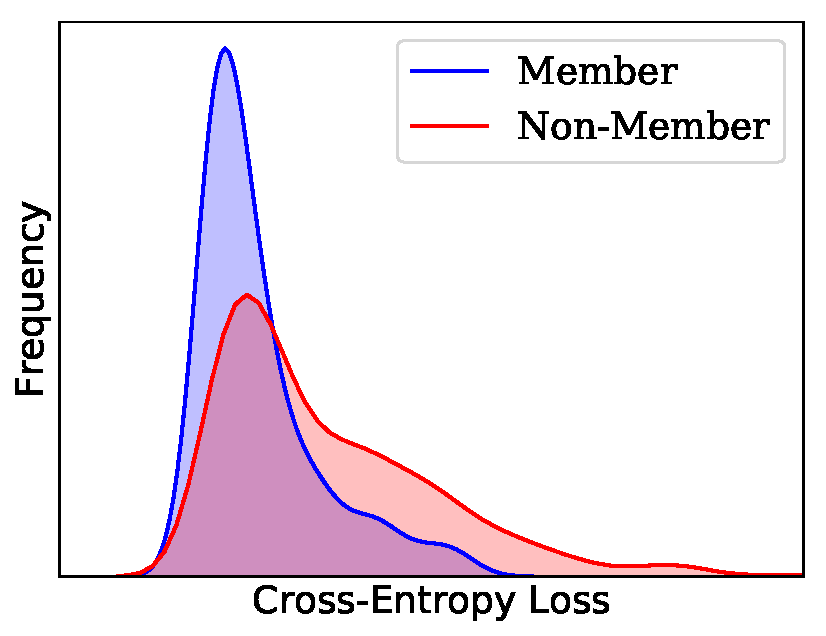
\includegraphics[width=0.5\linewidth]{figures/BBMIA/cora.pdf}}
    }

    \subfigure[Output Distribution for all records]{
    \label{fig:mem_soft_label}
    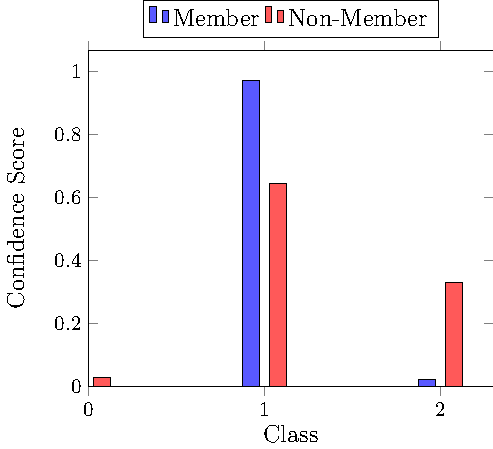
\includegraphics[width=0.5\linewidth]{figures/BBMIA/pubmed_hist.pdf}
    \raisebox{2mm}{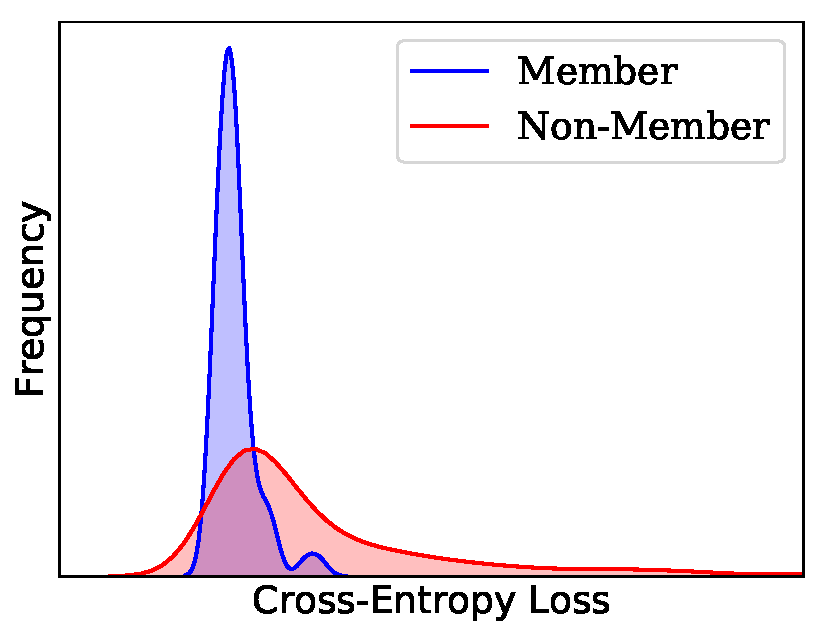
\includegraphics[width=0.5\linewidth]{figures/BBMIA/pubmed.pdf}}
    }
    \end{minipage}
    \caption{Distribution of the confidence score vectors of the target classifier on the training data and test data of class 29 in the Purchase100 dataset. Each color represents one data record.}
    \label{fig:soft_label}
\end{figure}


\textbf{Impact of Increasing Number of Layers}

\begin{figure}[!htb]
\centering
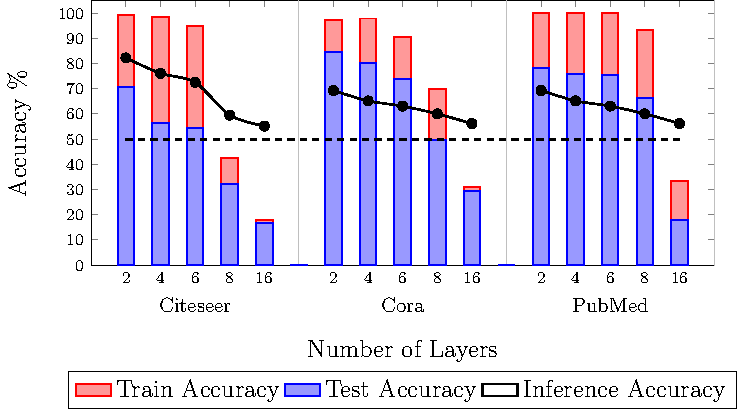
\includegraphics[width=0.5\textwidth]{./figures/BBMIA/gsage_numlayers.pdf}
\caption{Example of a parametric}
\end{figure}

We evaluate the performance of confidence attack on increasing the range of neighbourhood nodes used for aggregating the features (Figure~\ref{fig:numlayers}).
To do that, we extend the range of the message passing algorithm by increasing the number of layers in the GNNs~\cite{klicpera2018combining,Li2018DeeperII}.
% to indicate whether the neighbourhood nodes in structured graph data influence the membership inference accuracy (Figure~\ref{fig:numlayers}).
%The range of the message passing algorithm can be extended by increasing the number of layers in the GNNs~\cite{klicpera2018combining,Li2018DeeperII}.
On increasing the number of layers from 2 to 6, the inference accuracy decreases by 16\% for TAGCN, 8\% for GCN, GraphSAGE and GAT despite a small decrease of 3\% in test accuracy for Pubmed dataset.
Interestingly, the generalization error increases (train accuracy remains the same but the test accuracy decreases) for Cora, Citeseer and Pubmed, but the inference accuracy continues to decrease which indicates that the influence of preferential connections between different nodes in the graph plays a significant role in influencing the inference accuracy. % than the generalization error.
%\textbf{indicates the influence of preferential connections between different nodes in the graph play a significant role in influencing the inference accuracy than the generalization error}.
For large number of layers ($>$ 8 layers) in the GNN, for all the datasets and architectures, the model completely loses it's predictive power.
In general, the inference accuracy as well as prediction accuracy decreases with increasing the range of the message passing algorithm by increasing the layers from 2 to 16.
This implies that the membership privacy leakage is influenced by the structured graph data with preferential connections between different nodes.
%\textbf{This implies that the membership privacy leakage is influenced by the structured graph data with preferential connections between different nodes.}
Specifically, aggregating features from larger number of nodes results in higher averaging which reduces the distinguishability (over-smoothening of features) as model converges to random walk’s limit distribution~\cite{klicpera2018combining,Li2018DeeperII} which is crucial for inference attacks~\cite{7958568,ndss19salem}.
Further, at 16 layers the model is underfitting despite which we see an inference attack accuracy of 57\% on average above the random guess which is still significant.
This indicates that reducing the generalization error of GNNs is not enough to mitigate the inference attack risks.
%\textbf{This indicates that reducing the generalization error of GNNs is insufficient to mitigate the inference attack risks.}
In summary, overfitting is not the sole cause for membership inference attacks in GNNs and the message passing algorithm which aggregates features from neighbouring nodes (which captures preferential connections) contributes as well.







\subsection{Whitebox Inference Attack}

We exploit the difference in intermediate feature representation of train and test data to perform membership inference attack in a whitebox setting (Table~\ref{whitebox}).
Results show that different models trained on PubMed dataset leak significantly more information between 20\% and 36\% over random guess accuracy.
On the other hand, models trained on Citeseer dataset provide to the adversary an advantage between ~7\% and ~17\% over random guess while for Cora dataset it is between 4\% and 7\%.
The embedding is significantly different for train and test data points for PubMed dataset as seen Figure~\ref{embedding}(a) which result in a higher whitebox membership inference accuracy compared to Cora and Citeseer dataset (Figure~\ref{embedding}(b) and (c)).
The higher accuracy for Pubmed dataset can be attributed to significant distinguishability of features as seen by visually inspecting in Figure~\ref{embedding}.


\begin{figure}
    \centering
    \begin{minipage}[b]{1\linewidth}
    \centering
    \subfigure[Train data]{
   	\label{fig:mem_soft_label}
    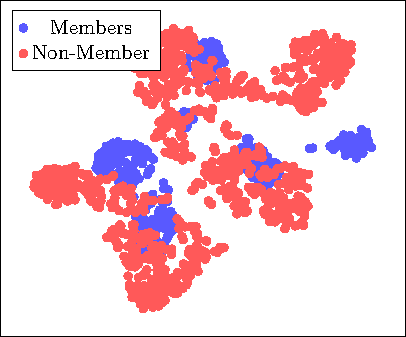
\includegraphics[width=0.5\linewidth,height=3.5cm, keepaspectratio]{figures/EmbeddingMIA/citeseer.pdf}
    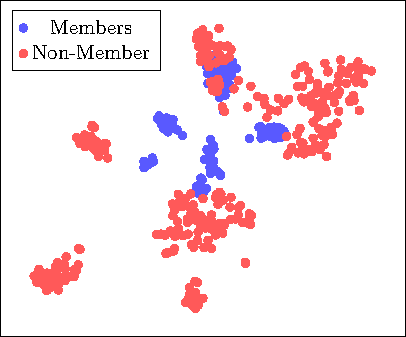
\includegraphics[width=0.5\linewidth,height=3.5cm, keepaspectratio]{figures/EmbeddingMIA/cora.pdf}
    }

    \subfigure[Train data]{
    \label{fig:mem_soft_label}
    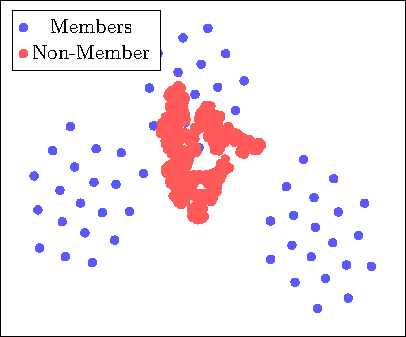
\includegraphics[width=0.5\linewidth,height=3.5cm, keepaspectratio]{figures/EmbeddingMIA/pubmed.pdf}
    \raisebox{-2mm}{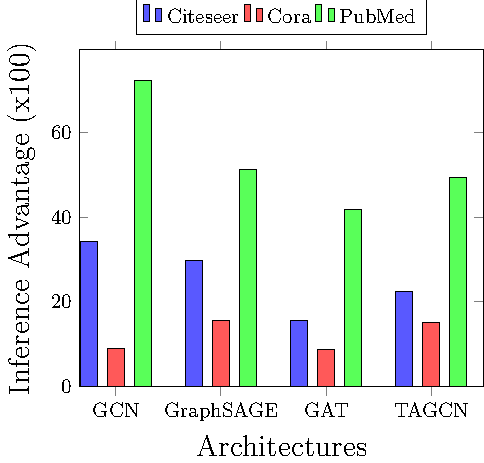
\includegraphics[width=0.5\linewidth]{figures/EmbeddingMIA/whiteboxMIA.pdf}}
    }
    \end{minipage}
    \caption{Distribution of the confidence score vectors of the target classifier on the training data and test data of class 29 in the Purchase100 dataset. Each color represents one data record.}
    \label{fig:soft_label}
\end{figure}



The success of the unsupervised whitebox attack is attributed to the message passing which updates the parameters (weights) to specifically ensure higher distinguishability between the data points of different classes for high accuracy on training dataset.
Indeed, the parameters are specifically updated to fit the training dataset resulting in a high distinguishability between feature embedding of train and test data records.
Moreover, the feature embedding for the initial layers are useful since for later layers the features are oversmoothened which also reduces accuracy (as seen in increasing the range of nodes of message passing algorithm).




\subsection{Reconstruction Attack}

We compute the



Cora testroc= 0.65075 testap= 0.72299
Citeseer testroc= 0.71344 testap= 0.77835

Increase Adversary Knowledge to 50% train: Cora: testroc= 0.76476 testap= 0.81545
Citeseer: testroc= 0.77927 testap= 0.82840

\begin{figure}[!htb]
    \centering
    \begin{minipage}[b]{1\linewidth}
    \centering
    \subfigure[Validation ROC]{
   	\label{fig:mem_soft_label}
    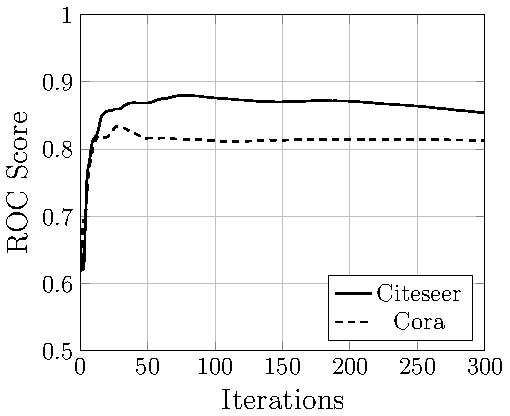
\includegraphics[width=0.5\linewidth]{figures/Reconstruction/roc.pdf}
    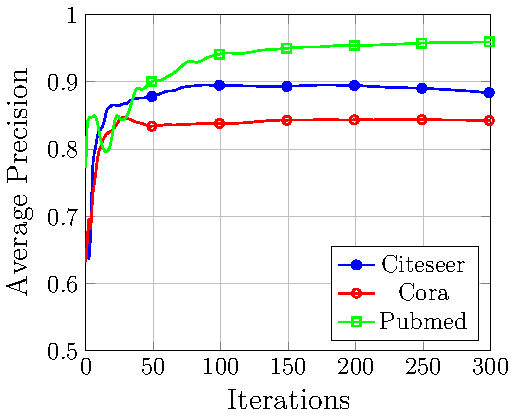
\includegraphics[width=0.5\linewidth]{figures/Reconstruction/ap.pdf}
    }
    \end{minipage}
    \caption{Distribution of the confidence score vectors of the target classifier on the training data and test data of class 29 in the Purchase100 dataset. Each color represents one data record.}
    \label{fig:soft_label}
\end{figure}

\subsection{Stealing Model Functionality}


\subsection{Link Inference Attack}

\begin{wrapfigure}{l}{0.5\linewidth}
  \begin{center}
    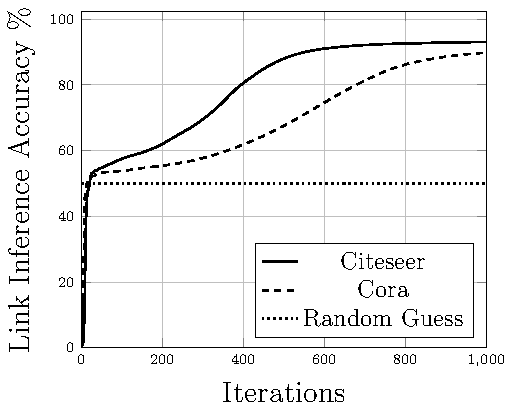
\includegraphics[width=\linewidth]{figures/LinkInfer/LinkInfer.pdf}
  \end{center}
  \caption{Birds}
\end{wrapfigure}


Link inference attack is a binary classification problem and the accuracy of random guess is 50\%.
Hence, an accuracy beyond 50\% indicates that the adversary has an added advantage to infer the links between two nodes.
For Citeseer dataset, the accuracy of of inference is around 93.39\% while for Cora dataset the inference accuracy is 90.73\%.
The above results are assuming a practical adversary setting with 1585 training data points (30\%) compared to 3166 test data points (60\%) and 527 validation data points (10\%) for Cora dataset.
The same train-test-validation distribution is used for Citeseer dataset with 1366 (30\%) train records, 2731 (60\%) test records and 455 (10\%) validation records.



\subsection{Attribute Inference Attack}

In case of attribute inference attacks, we evaluate two state of the art embedding models: Node2Vec and DeepWalk.
We generate embeddings using the two algorithms on Facebook and LastFM dataset which contain gender and location as senstivie attributes respectively.


\begin{figure}
    \centering
    \begin{minipage}[b]{1\linewidth}
    \centering
    \subfigure[Train data]{
   	\label{fig:mem_soft_label}
    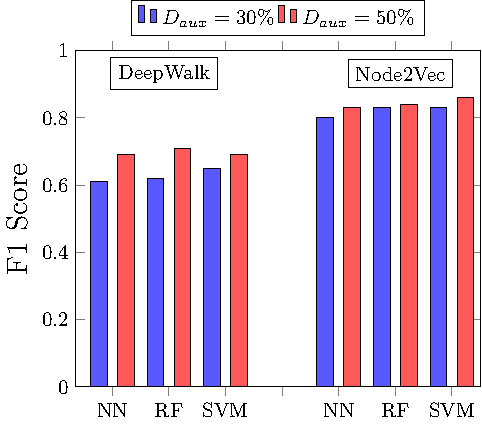
\includegraphics[width=0.5\linewidth,height=3.5cm, keepaspectratio]{./figures/AIA/lfm_AIA.pdf}
    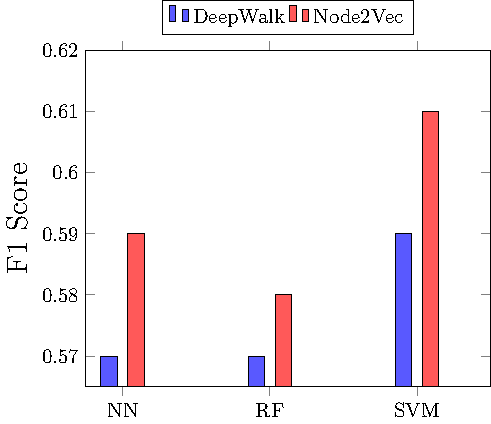
\includegraphics[width=0.5\linewidth,height=3.5cm, keepaspectratio]{./figures/AIA/fb_AIA.pdf}
    }

    \end{minipage}
    \caption{Distribution of the confidence score vectors of the target classifier on the training data and test data of class 29 in the Purchase100 dataset. Each color represents one data record.}
    \label{fig:soft_label}
\end{figure}

FB: (DeepWalk)
NN  0.57
RF 0.58
SVM 0.59

FB Node2Vec
NN 0.59
Rf 0.57
SVM 0.61

\textbf{Impact of Adversary's Knowledge.}

50\% knowlege

LFM (DeepWalk)
NN 0.69
RF 0.71
SVM 0.69


Node2Vec
LFM
NN:0.83
RF:0.84
SVM: 0.86
